% ============================================================
%  CSL7360 Computer Vision - Assignment 2 report
%  Cost-Efficient Salient Object Segmentation
%  Compile: latexmk -pdf -interaction=nonstopmode -halt-on-error report.tex
% ============================================================
\documentclass[10pt,a4paper,twocolumn]{article}

\usepackage[a4paper,top=1.9cm,bottom=1.8cm,left=1.6cm,right=1.6cm,columnsep=0.7cm]{geometry}
\usepackage[T1]{fontenc}
\usepackage[utf8]{inputenc}
\usepackage{mathpazo}
\usepackage[scaled=0.92]{helvet}
\usepackage{microtype}
\usepackage{amsmath,amssymb}
\usepackage{graphicx}
\usepackage{booktabs,array,multirow}
\usepackage[table]{xcolor}
\usepackage{tikz}
\usetikzlibrary{arrows.meta,positioning,calc,backgrounds}
\usepackage{enumitem}
\usepackage{caption}
\usepackage{titlesec}
\usepackage{fancyhdr}
\usepackage{balance}
\usepackage[colorlinks=true,linkcolor=navy,urlcolor=teal,citecolor=navy]{hyperref}

% ---------- palette ----------
\definecolor{navy}{HTML}{1F3A5F}
\definecolor{teal}{HTML}{2A9D8F}
\definecolor{amber}{HTML}{E9A23B}
\definecolor{coral}{HTML}{E76F51}
\definecolor{paper}{HTML}{F4F7FA}
\definecolor{rule}{HTML}{C9D3DE}

% ---------- CPU used for the reported timing run ----------
\newcommand{\cpumodel}{\texttt{11th Gen Intel(R) Core(TM) i5-11400H @ 2.70 GHz}}

% ---------- typography ----------
\setlength{\parindent}{0pt}
\setlength{\parskip}{0.42em}
\linespread{1.03}
\setlist{nosep,leftmargin=1.2em,itemsep=1pt}
\captionsetup{font={small},labelfont={bf,color=navy},labelsep=period,skip=4pt}

\titleformat{\section}{\sffamily\large\bfseries\color{navy}}{\thesection}{0.6em}{}[{\color{rule}\titlerule[0.6pt]}]
\titleformat{\subsection}{\sffamily\normalsize\bfseries\color{teal}}{\thesubsection}{0.5em}{}
\titlespacing*{\section}{0pt}{1.1em}{0.5em}
\titlespacing*{\subsection}{0pt}{0.8em}{0.3em}

\setlength{\headheight}{19pt}
\pagestyle{fancy}
\fancyhf{}
\renewcommand{\headrulewidth}{0.4pt}
\renewcommand{\headrule}{\hbox to\headwidth{\color{rule}\leaders\hrule height \headrulewidth\hfill}}
\fancyhead[L]{\sffamily\footnotesize\color{navy}CSL7360 -- Computer Vision \,|\, Assignment 2}
\fancyhead[R]{\sffamily\footnotesize\color{navy}Prasangeet\ Dongre \,(B23CH1033)}
\fancyfoot[C]{\sffamily\footnotesize\thepage}

\newcommand{\Tcpu}{T_{\mathrm{CPU}}}
\newcommand{\Sdisk}{S_{\mathrm{disk}}}
\newcommand{\key}[2]{\begin{tabular}{@{}c@{}}{\sffamily\bfseries\large\color{navy}#1}\\[-1pt]{\sffamily\scriptsize\color{gray}#2}\end{tabular}}

\begin{document}

% ============================================================
%  Title block (spans both columns)
% ============================================================
\twocolumn[{%
\begin{center}
{\sffamily\bfseries\fontsize{19}{22}\selectfont\color{navy} Cost-Efficient Salient Object Segmentation\par}
\vspace{0.3em}
{\sffamily\large\color{teal} A 176K-parameter residual U-Net under a 50\,ms single-core CPU budget\par}
\vspace{0.6em}
{\sffamily\bfseries Prasangeet Dongre} \quad {\sffamily\small(Roll No.\ B23CH1033)}\\[1pt]
{\sffamily\small B.Tech Chemical Engineering, IIT Jodhpur \,\textbullet\, CSL7360 Computer Vision, Assignment 2 (Track B)}
\end{center}
\vspace{0.2em}
\noindent\colorbox{paper}{%
\parbox{\dimexpr\textwidth-2\fboxsep}{%
\vspace{3pt}
\centering
\key{0.749}{mIoU (DUTS-TE)}\hspace{1.6em}%
\key{0.519}{Boundary F1}\hspace{1.6em}%
\key{0.680}{quality $Q$}\hspace{1.6em}%
\key{17.3 ms}{$\Tcpu$ per image}\hspace{1.6em}%
\key{0.73 MiB}{$\Sdisk$}\hspace{1.6em}%
\key{0.6205}{CES}
\vspace{3pt}}}
\vspace{0.6em}

\noindent{\sffamily\bfseries\color{navy}Abstract.}\;
We build a binary salient-object segmenter that has to label every pixel of a $256{\times}256$ photograph within 50\,ms of single-thread CPU time and a 4\,MiB parameter file. Our model is a three-level residual U-Net with a dilated depthwise multi-scale context block at the bottleneck and deep supervision, trained from scratch on DUTS-TR at $128{\times}128$ working resolution. On the full DUTS-TE benchmark (5{,}019 images) it reaches mIoU\,=\,0.7491, Boundary F1\,=\,0.5192 and $Q$\,=\,0.6801 at $\Tcpu$\,=\,17.32\,ms with a 767{,}807-byte checkpoint, giving CES\,=\,0.6205. On eleven hand-annotated photographs from our surroundings it reaches aggregate mIoU\,=\,0.8484 and quality $Q$\,=\,0.7732. The custom set is a small supplementary stress test, not a substitute for the official benchmark; its difficult scenes expose remaining weaknesses in contour accuracy and clutter handling.
\vspace{0.8em}
}]

% ============================================================
\section{Introduction}
The assignment asks for a pipeline that separates the salient foreground object from the background. Fully convolutional networks provide a natural formulation for dense, pixel-wise prediction, while encoder--decoder architectures use skip connections to combine coarse semantic features with finer spatial information \cite{long2015fcn,ronneberger2015unet}. The present work adapts these ideas to a strict CPU-time and model-size budget. The system is scored by
\begin{equation}
Q = 0.70\,\mathrm{mIoU} + 0.30\,\mathrm{BF1},
\end{equation}
\begin{equation}
\mathrm{CES} = Q\Bigl(1-0.20\tfrac{\Tcpu}{50\,\mathrm{ms}}-0.10\min\bigl(1,\tfrac{\Sdisk}{4\,\mathrm{MiB}}\bigr)\Bigr),
\end{equation}
with CES set to zero if $\Tcpu>50$\,ms. We follow \emph{Track B} (a small fully convolutional network written and trained from scratch). The design question is therefore twofold: how accurate can a network be, and how little of the time and storage budget does it need to spend to get there? Both penalty terms are linear, so each millisecond costs $0.4\%$ of $Q$ and the whole file-size term at most $10\%$. A model that is accurate \emph{and} tiny wins over a bigger, slightly more accurate one.

% ============================================================
\section{Data and Preprocessing}
\subsection{Splits}
The experiments use the DUTS salient-object dataset, which provides separate training and test partitions for salient-object detection \cite{wang2017duts,dutswebsite}. DUTS-TR (10{,}553 images) is split into a training and a validation part; DUTS-TE (5{,}019 images) is the final benchmark. The validation set is $10\%$ of DUTS-TR, drawn deterministically (seed 42) and stratified by foreground area: images are sorted by the fraction of mask pixels that are object, cut into strata, and sampled within each stratum, so that small and large objects appear in both parts in similar proportions.

\begin{table}[h]
\centering\small
\begin{tabular}{@{}lrl@{}}
\toprule
\textbf{Split} & \textbf{Images} & \textbf{Use}\\
\midrule
DUTS-TR (train) & 9{,}498 & gradient updates\\
DUTS-TR (val)   & 1{,}055 & monitoring, checkpoint choice\\
DUTS-TE         & 5{,}019 & final benchmark\\
Own photos      & 11 & supplementary test only\\
\bottomrule
\end{tabular}
\caption{Dataset splits.}
\end{table}

\textbf{Test-set hygiene.} DUTS-TE is not loaded by the training loop, contributes no gradient updates, and is not used for within-run checkpoint selection. However, DUTS-TE results were inspected during iterative comparisons of candidate designs. The test set must therefore not be described as a completely untouched blind set. The number reported here is the final evaluation run under the protocol described below.

\subsection{Preprocessing and augmentation}
Training and validation use the \texttt{DUTSDataset} loader, which resizes each original DUTS-TR photograph directly to $128{\times}128$ with \texttt{cv2.INTER\_AREA} and each mask to $128{\times}128$ with \texttt{cv2.INTER\_NEAREST}. A mask pixel is foreground when its grayscale value is at least 128. The official DUTS-TE evaluator follows a separate path: it prepares the photograph and mask at $256{\times}256$ outside the timed region, downsamples the photograph to the model's $128{\times}128$ working resolution inside the timed region, then upsamples logits and computes metrics at $256{\times}256$. Captured photographs are also prepared at $256{\times}256$ and paired with manually annotated masks, which are thresholded at 128 to make binary targets. Inputs are converted from BGR to RGB and normalized to $[0,1]$. During DUTS-TR training only, image and mask receive the same random horizontal flip ($p{=}0.5$), vertical flip ($p{=}0.10$) and isotropic rescaling by $0.9$--$1.1$ ($p{=}0.5$, new border pixels are background); the image alone additionally gets brightness and per-channel gain jitter with clipping.

% ============================================================
\section{Method}
\subsection{Architecture}
The network (Fig.~\ref{fig:arch}) is a compact, three-level residual U-Net with 175{,}971 trainable parameters. Its encoder--decoder organization and skip connections follow the general design principles of U-Net and fully convolutional segmentation networks \cite{ronneberger2015unet,long2015fcn}; the residual blocks use identity or projected shortcuts in the spirit of residual learning \cite{he2016resnet}. Each encoder block has two $3{\times}3$ convolutions with batch normalization and ReLU, plus a projected residual shortcut when the channel counts differ. Channel widths are deliberately narrow, $16\!\to\!24\!\to\!40\!\to\!56$, and max pooling halves the spatial resolution between stages.

\textbf{Dilated multi-scale context.} Salient objects range from a computer mouse to a whole backpack, so the bottleneck (at $1/8$ of the working resolution) needs several receptive-field sizes. Three parallel branches, each a $1{\times}1$ projection to 16 channels followed by a \emph{depthwise} $3{\times}3$ convolution with dilation 1, 2 and 4, are concatenated, projected back to 56 channels and added to the bottleneck input. Using several dilation rates follows the principle of multi-scale context aggregation with dilated convolutions \cite{yu2016dilated}. The depthwise operation is a parameter-efficient convolutional factorization used in lightweight network designs such as MobileNets \cite{howard2017mobilenets}; here it keeps the contextual branches small.

\textbf{Decoder and skips.} The decoder upsamples, concatenates the matching encoder feature (U-Net style skip connections) and applies a residual block: $56{+}40\!\to\!40$, $40{+}24\!\to\!24$, $24{+}16\!\to\!16$. A final $1{\times}1$ convolution gives one logit per pixel. Two auxiliary $1{\times}1$ heads on the quarter- and half-resolution decoder stages provide deep supervision during training, following the general idea of companion objectives at intermediate layers \cite{lee2015dsn}; at inference only the main head runs.

% ---------- architecture figure (full width) ----------
\begin{figure*}[t]
\centering
\resizebox{\textwidth}{!}{%
\begin{tikzpicture}[
  blk/.style={draw=navy,fill=navy!10,rounded corners=2pt,minimum width=1.35cm,align=center,font=\sffamily\scriptsize,inner sep=2pt},
  enc/.style={blk,fill=navy!12},
  dec/.style={blk,fill=teal!16,draw=teal!80!black},
  ctx/.style={blk,fill=amber!25,draw=amber!80!black,minimum width=2.3cm},
  aux/.style={blk,fill=coral!15,draw=coral,dashed,minimum width=1.0cm,minimum height=0.55cm},
  flow/.style={-{Stealth[length=4pt]},thick,navy!70},
  skip/.style={-{Stealth[length=4pt]},thick,dashed,teal!70!black},
  lab/.style={font=\sffamily\scriptsize,text=black!60}]
\node[blk,fill=white,minimum height=1.9cm] (in) at (0,0) {RGB\\$128^2$\\$\times 3$};
\node[enc,minimum height=1.9cm] (e1) at (2.0,0) {Enc 1\\ResBlock\\\textbf{16}};
\node[enc,minimum height=1.45cm] (e2) at (4.0,-0.2) {Enc 2\\ResBlock\\\textbf{24}};
\node[enc,minimum height=1.05cm] (e3) at (6.0,-0.4) {Enc 3\\ResBlock\\\textbf{40}};
\node[ctx,minimum height=0.95cm] (bn) at (8.55,-0.55) {Bottleneck \textbf{56}\\dilated DW ctx\\$d\in\{1,2,4\}$};
\node[dec,minimum height=1.05cm] (d3) at (11.1,-0.4) {Dec 3\\ResBlock\\\textbf{40}};
\node[dec,minimum height=1.45cm] (d2) at (13.1,-0.2) {Dec 2\\ResBlock\\\textbf{24}};
\node[dec,minimum height=1.9cm] (d1) at (15.1,0) {Dec 1\\ResBlock\\\textbf{16}};
\node[blk,fill=white,minimum height=1.9cm] (out) at (17.1,0) {$1{\times}1$\\conv\\mask\\$128^2$};
\draw[flow] (in)--(e1); \draw[flow] (e1)--node[lab,above]{pool}(e2);
\draw[flow] (e2)--node[lab,above]{pool}(e3); \draw[flow] (e3)--node[lab,above]{pool}(bn);
\draw[flow] (bn)--node[lab,above]{up}(d3); \draw[flow] (d3)--node[lab,above]{up}(d2);
\draw[flow] (d2)--node[lab,above]{up}(d1); \draw[flow] (d1)--(out);
\draw[skip] (e1.north) to[out=50,in=130] node[lab,above]{skip (concat)} (d1.north);
\draw[skip] (e2.north) to[out=50,in=130] (d2.north);
\draw[skip] (e3.north) to[out=50,in=130] (d3.north);
\node[aux,above=0.55cm of d3] (a3) {aux $\tfrac14$};
\node[aux,above=0.62cm of d2] (a2) {aux $\tfrac12$};
\draw[dashed,coral,-{Stealth[length=3pt]}] (d3.north)--(a3.south);
\draw[dashed,coral,-{Stealth[length=3pt]}] (d2.north)--(a2.south);
\node[lab,anchor=north west] at (14.0,-1.55) {\textcolor{coral}{aux heads: training only}};
\end{tikzpicture}}
\caption{Architecture of the final network (175{,}971 parameters). Numbers in bold are channel counts. The dashed teal arcs are U-Net skip connections that concatenate encoder features into the decoder; the coral heads provide deep supervision during training and are removed at inference.}
\label{fig:arch}
\end{figure*}

\subsection{Loss and training}
Every supervised output uses an equal mix of binary cross-entropy (with logits) and soft Dice loss. Dice-based objectives have been used in segmentation to optimize overlap directly and to mitigate foreground--background imbalance \cite{milletari2016vnet}. The combined loss is
\begin{equation}
\mathcal{L}_{\text{base}} = 0.5\,\mathcal{L}_{\text{BCE}} + 0.5\,\mathcal{L}_{\text{Dice}},
\end{equation}
and deep supervision weights the main and auxiliary outputs as
\begin{equation}
\mathcal{L} = 0.60\,\mathcal{L}_{\text{main}} + 0.15\,\mathcal{L}_{1/4} + 0.25\,\mathcal{L}_{1/2}.
\end{equation}
The BCE term provides a per-pixel classification objective, while the Dice term emphasizes region overlap and helps counter the foreground--background imbalance. The chosen 50:50 weighting is an experimental setting for this model, not a value prescribed by the cited work.

We train from scratch (no pretrained weights) with AdamW, which decouples weight decay from the adaptive gradient update \cite{loshchilov2019adamw}, for 60 epochs on a GPU, batch size 8 with 2 accumulation steps (effective 16), peak learning rate $7{\times}10^{-4}$, 3 epochs of linear warm-up followed by cosine decay to $10^{-6}$, weight decay $10^{-5}$ (not applied to biases and normalisation parameters), gradient clipping at 1.0 and mixed precision. The checkpoint is chosen by validation quality $Q_{\text{val}}=0.70\,\mathrm{mIoU}+0.30\,\mathrm{BF1}$, which peaked at epoch 56 (Fig.~\ref{fig:curves}).

\begin{figure}[t]
\centering
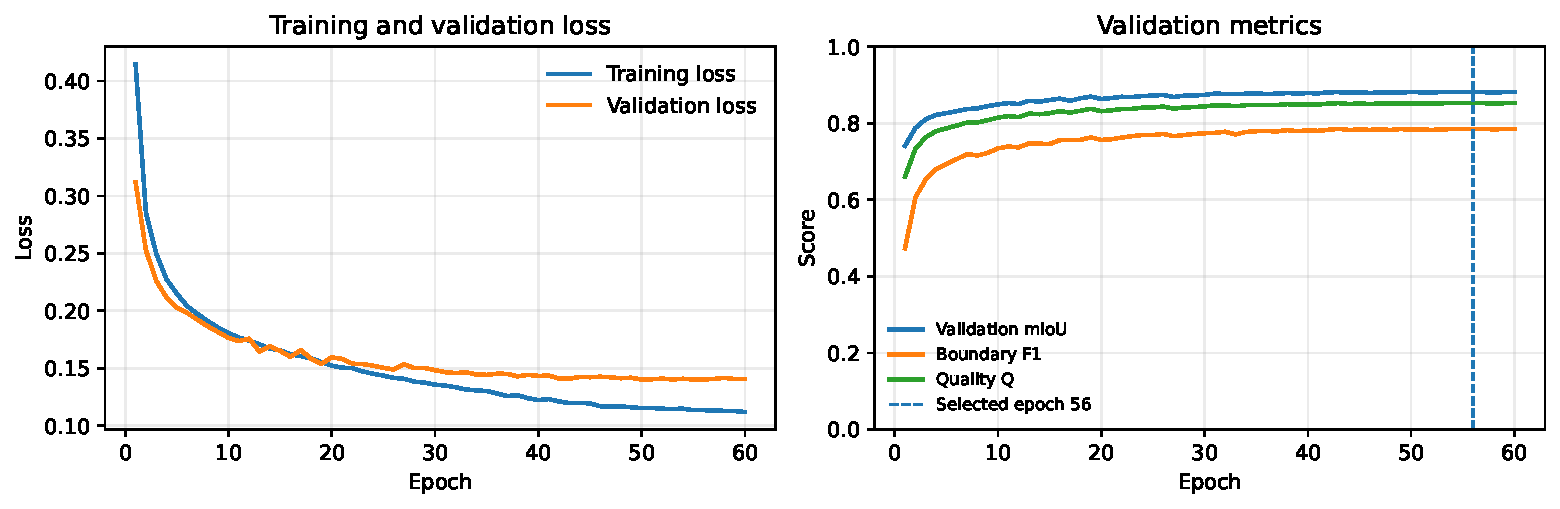
\includegraphics[width=\columnwidth]{figs/curves.pdf}
\caption{Training history. Left: training and validation loss. Right: validation mIoU, Boundary F1 and $Q$ (dashed line: selected epoch 56).}
\label{fig:curves}
\end{figure}

% ============================================================
\section{Keeping the Pipeline Fast}
The timed region starts with a $256{\times}256$ BGR photograph in memory and ends with a $256{\times}256$ array of 0s and 1s. Inside it we:
\begin{enumerate}
\item downscale to $128{\times}128$ with \texttt{INTER\_AREA},
\item convert BGR$\to$RGB, scale to $[0,1]$ and build the tensor,
\item run the network,
\item bilinearly upsample the logits to $256{\times}256$,
\item apply a sigmoid, threshold at 0.5 and materialise the NumPy mask.
\end{enumerate}
File I/O, resizing the original photograph to $256{\times}256$, loading the checkpoint and metric computation lie outside the timer. The main levers on cost were:
\begin{itemize}
\item \textbf{Half working resolution.} Running the CNN at $128{\times}128$ rather than $256{\times}256$ cuts the number of pixels processed by 4$\times$; the logits are upsampled afterwards.
\item \textbf{Very narrow channels} (16--56) and a context block built from depthwise convolutions.
\item \textbf{No test-time extras:} no ensembling, no flip averaging, no auxiliary heads at inference.
\item \textbf{Strict single-thread setup.} The four thread environment variables are set to \texttt{"1"} before importing NumPy, OpenCV or PyTorch, followed by \texttt{cv2.setNumThreads(1)} and \texttt{torch.set\_num\_threads(1)}; the model is warmed up once before timing.
\end{itemize}
$\Tcpu$ is the total \texttt{time.process\_time()} over all 5{,}019 DUTS-TE images divided by 5{,}019. The storage side is equally simple: the saved file is a plain, uncompressed PyTorch state dict of 767{,}807 bytes (0.7322\,MiB, 18.3\% of the 4\,MiB budget), all learned values live in it, and none are hard-coded.

\textbf{Evaluation implementation.} The official \texttt{src/evaluate.py} computes a four-connected foreground boundary and matches boundary pixels within a $5{\times}5$ neighbourhood (radius 2) using OpenCV \texttt{filter2D}. Constant-zero borders make pixels outside the image count as background. The helper in \texttt{src/metrics.py} implements the corresponding neighbourhood operations with NumPy slicing. For both paths, mIoU is derived from one aggregate $2{\times}2$ confusion matrix, while Boundary F1 is computed per image and then averaged. This is the project evaluation protocol; the tolerance radius is fixed at two pixels. Boundary evaluation is sensitive to the matching tolerance and annotation quality; the adopted neighbourhood and border convention are therefore stated explicitly rather than treating Boundary F1 as a protocol-independent quantity \cite{hou2013boundary}.

% ============================================================
\section{Results}
\begin{figure*}[!t]
\centering
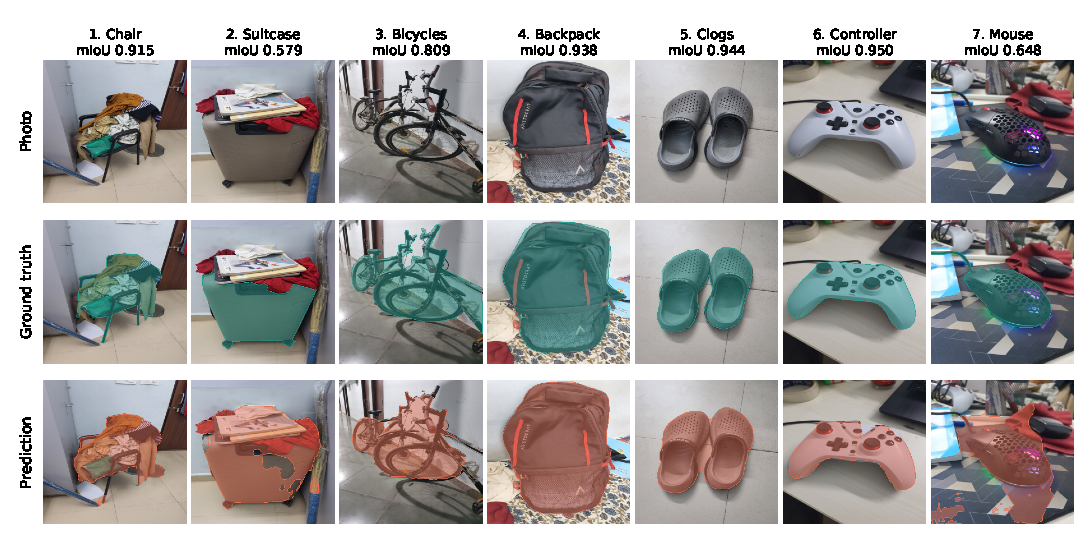
\includegraphics[width=\textwidth]{figs/captured.pdf}
\caption{Own photographs: input, ground-truth overlay (teal) and predicted overlay (coral), with per-image mIoU. All eleven paired photographs are shown, including difficult examples.}
\label{fig:captured}
\end{figure*}

\textbf{Hardware.} All timings were measured on CPU only, with one thread, using PyTorch and OpenCV. CPU: \cpumodel.

\begin{table*}[t]
\centering\small
\renewcommand{\arraystretch}{1.18}
\begin{tabular}{@{}lcccccccc@{}}
\toprule
\textbf{Set} & \textbf{Images} & \textbf{Res.} & \textbf{mIoU} & \textbf{BF1} & \textbf{$Q$} & \textbf{$\Tcpu$ (ms)} & \textbf{$\Sdisk$ (bytes)} & \textbf{CES}\\
\midrule
Validation (DUTS-TR split) & 1{,}055 & $128^2$\textsuperscript{a} & 0.8819 & 0.7854 & 0.8529 & -- & 767{,}807 & --\\
\rowcolor{paper}
\textbf{DUTS-TE (official)} & 5{,}019 & $256^2$ & \textbf{0.7491} & \textbf{0.5192} & \textbf{0.6801} & \textbf{17.32} & \textbf{767{,}807} & \textbf{0.6205}\\
Own photos & 11 & $256^2$ & 0.8484 & 0.5978 & 0.7732 & 17.14\textsuperscript{b} & 767{,}807 & --\\
\bottomrule
\end{tabular}
\caption{Main results. mIoU is computed from one aggregate confusion matrix; BF1 is the mean of per-image scores. \textsuperscript{a}Validation numbers come from the 128$\times$128 training loop and are therefore not resolution-matched with the $256{\times}256$ test numbers. \textsuperscript{b}Mean over 220 timed predictions (20 per photograph after one warm-up); the official $\Tcpu$ is the DUTS-TE average. CES is reported only for DUTS-TE, the common benchmark.}
\label{tab:main}
\end{table*}

\subsection{DUTS-TE benchmark}
\begin{figure}[!t]
\centering
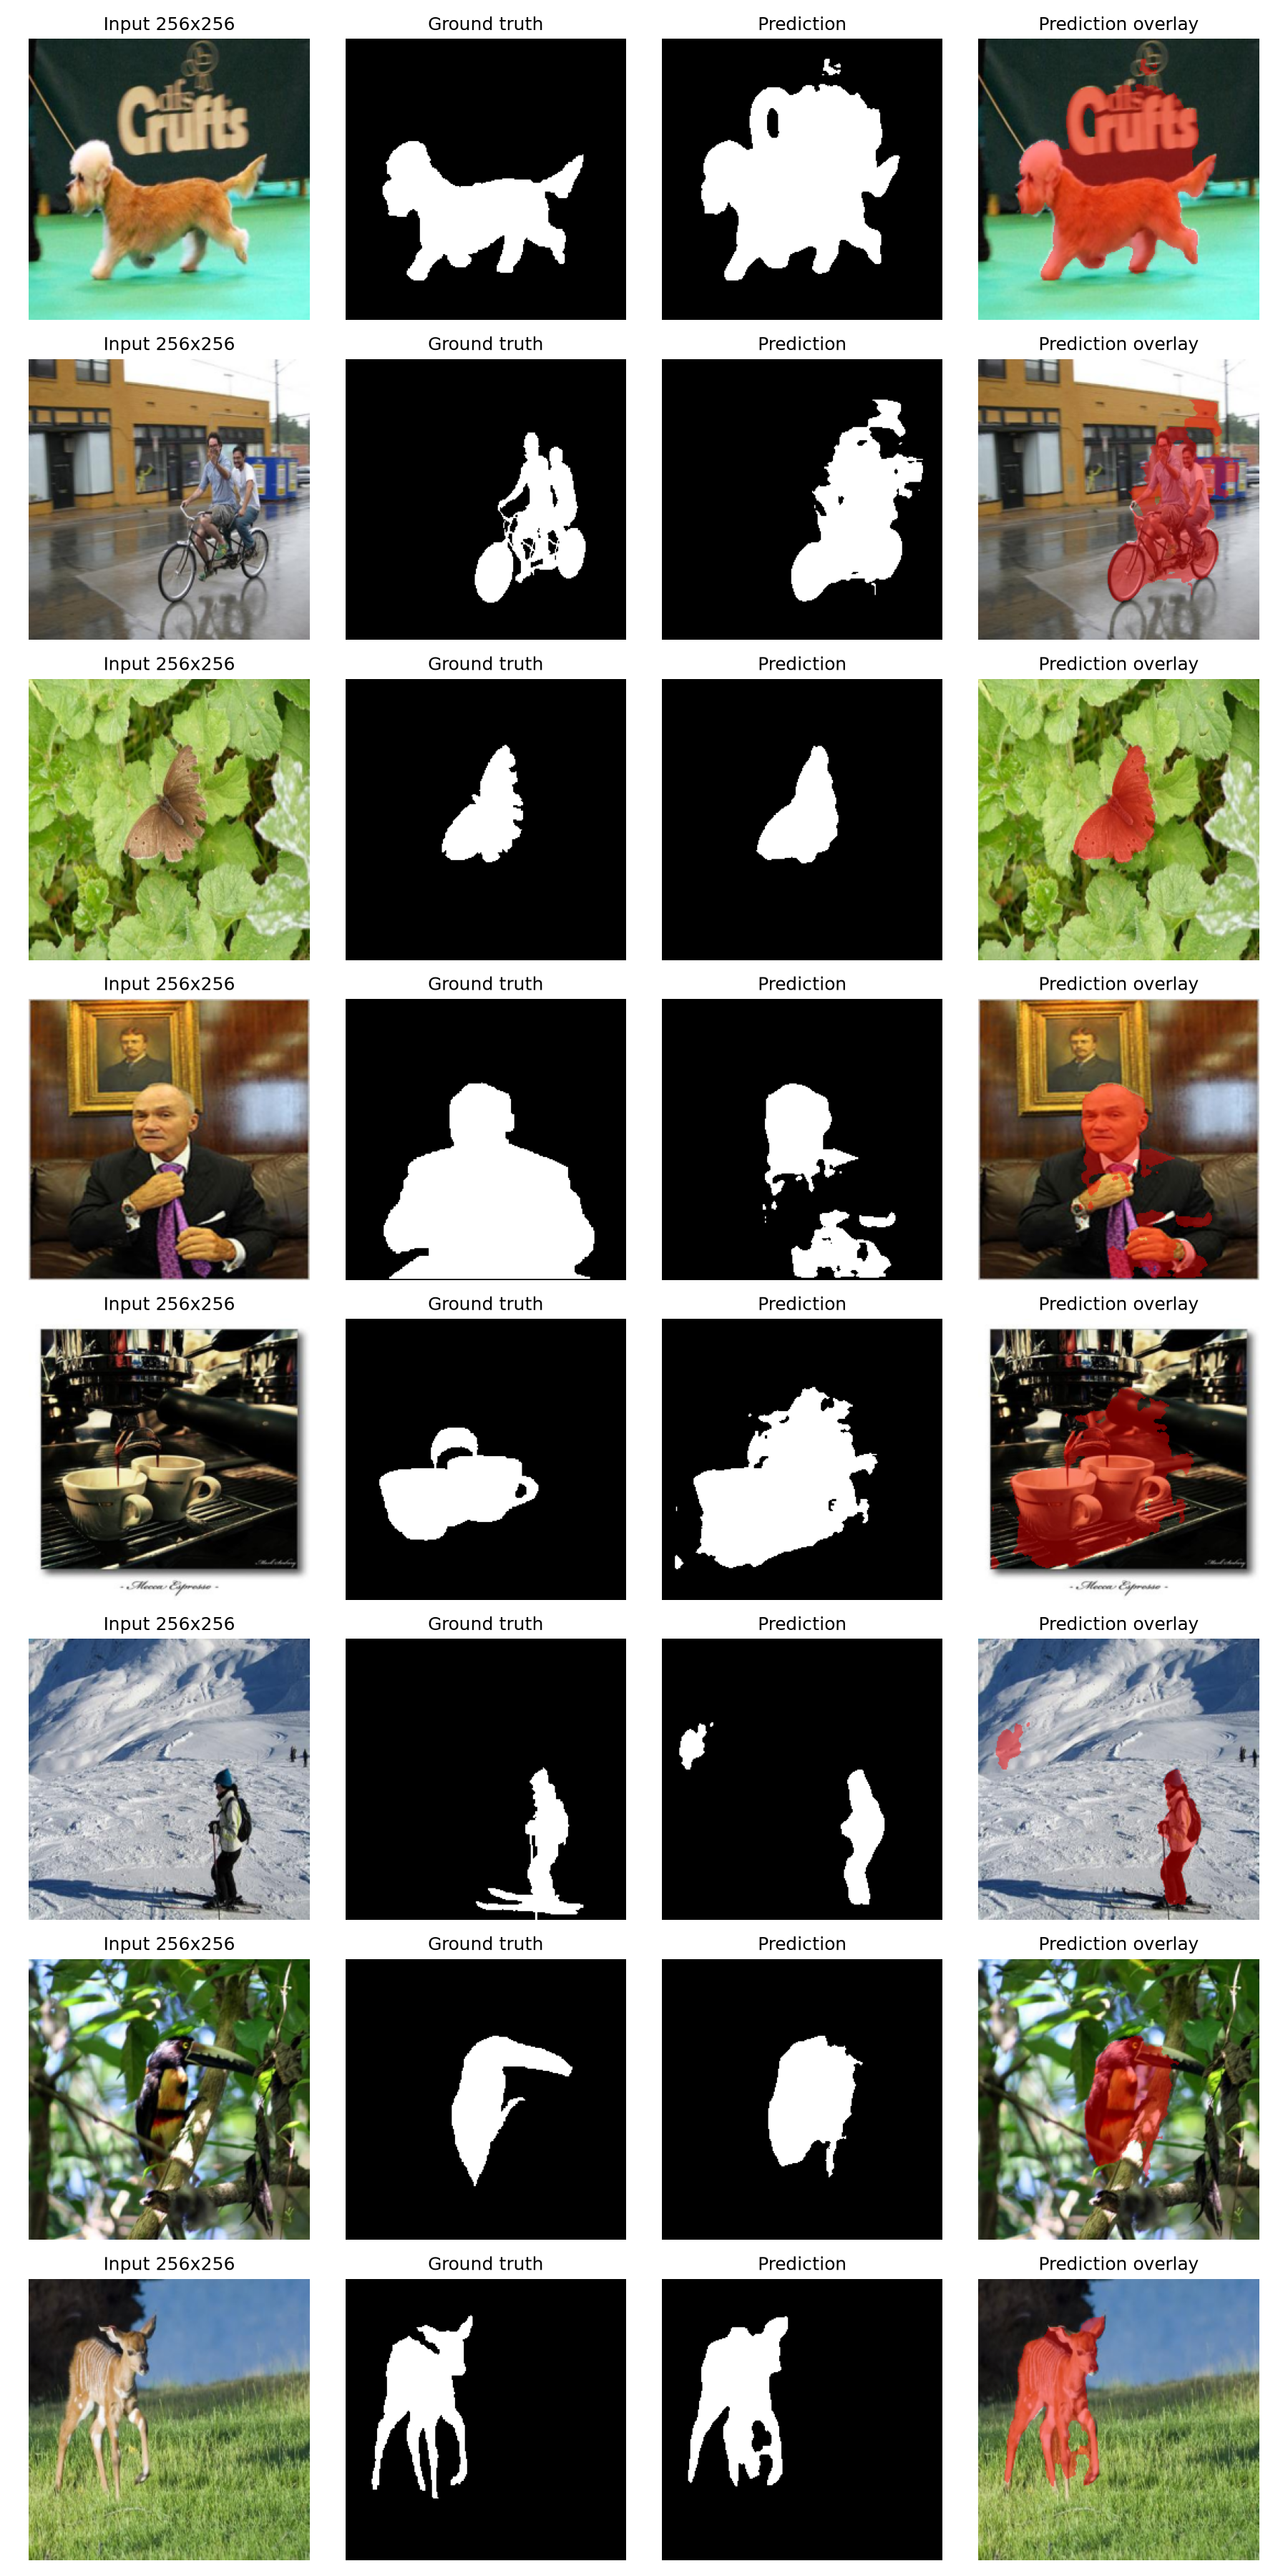
\includegraphics[width=0.8\columnwidth]{figs/duts.png}
\caption{DUTS-TE examples (input, ground truth, prediction). Good: butterfly, fawn. Failures: the seated man (large object, dark clothing blending with the sofa) and the skier (small object, spurious blob on the snow).}
\label{fig:duts}
\end{figure}
Table~\ref{tab:main} summarises all three evaluation sets. On DUTS-TE the pipeline spends 17.32\,ms per image (34.6\% of the time budget), so both hard limits are met with room to spare and the efficiency penalty is only
\[
\bigl(1-0.20\cdot\tfrac{17.32}{50}-0.10\cdot\tfrac{767807}{4194304}\bigr)=0.9124 .
\]
Hence $\mathrm{CES}=0.6801\times0.9124=0.6205$.

Background IoU (0.9106) is far higher than foreground IoU (0.5875): the aggregate confusion matrix shows $14.5$M background pixels wrongly marked as object but also $11.6$M object pixels missed, against $37.1$M correctly found. Boundary F1 of 0.52 confirms that contours, more than regions, are the main weakness. Qualitative DUTS-TE examples are in Fig.~\ref{fig:duts}: compact, high-contrast objects (butterfly, fawn) are segmented well, while large objects in clutter (the seated man) and multi-part scenes are only partially recovered.

\textbf{Validation-to-test gap.} Validation $Q$ (0.853) is much higher than test $Q$ (0.680). Part of this is the resolution mismatch noted in Table~\ref{tab:main}, and part is likely that the validation split, drawn from the same distribution as the training data, is easier than the official test set; the gap should not be read as a clean estimate of overfitting.


\subsection{Own photographs}
We retained eleven everyday photographs and annotated each target by hand on the $256{\times}256$ prepared image. The set includes a chair/clothes composite, a suitcase, two bicycles, a backpack, clogs, a controller, a mouse, a bird, a cat at a window, a kitten and a wristwatch. It deliberately includes clutter, occlusion, small foreground regions and thin structures. Fig.~\ref{fig:captured} shows the input, ground-truth and predicted overlays; Table~\ref{tab:captured} gives per-image scores. These photographs were used only for supplementary testing.


\begin{table}[t]
\centering\small
\renewcommand{\arraystretch}{1.08}
\begin{tabular}{@{}cl>{\raggedleft\arraybackslash}p{0.95cm}>{\raggedleft\arraybackslash}p{0.85cm}>{\raggedleft\arraybackslash}p{0.85cm}@{}}
\toprule
\textbf{ID} & \textbf{Target} & \textbf{IoU$_{\text{fg}}$} & \textbf{mIoU} & \textbf{BF1}\\
\midrule
1 & Chair / clothes & 0.867 & 0.915 & 0.720\\
2 & Suitcase & 0.469 & 0.579 & 0.298\\
3 & Two bicycles & 0.747 & 0.809 & 0.445\\
4 & Backpack & 0.947 & 0.938 & 0.651\\
5 & Pair of clogs & 0.922 & 0.944 & 0.867\\
6 & Controller & 0.924 & 0.950 & 0.795\\
7 & Computer mouse & 0.503 & 0.648 & 0.165\\
8 & Bird & 0.930 & 0.960 & 0.867\\
9 & Cat at window & 0.570 & 0.768 & 0.435\\
10 & Kitten & 0.896 & 0.934 & 0.644\\
11 & Wristwatch & 0.897 & 0.940 & 0.689\\
\midrule
\multicolumn{2}{@{}l}{Aggregate} & 0.777 & 0.848 & 0.598\textsuperscript{c}\\
\bottomrule
\end{tabular}
\caption{Per-photo results. \textsuperscript{c}Mean per-image BF1; mean per-image mIoU is 0.853.}
\label{tab:captured}
\end{table}

Timing over 220 predictions averaged 17.1447\,ms (median 16.6661\,ms, std.\ 1.5790\,ms, min 14.5730\,ms, max 22.2957\,ms). These repeated timings are supplementary and do not replace the official DUTS-TE timing.

% ============================================================
\section{Failure Analysis}
\textbf{Suitcase (ID 2): occlusion and internal detail.} This is the weakest region-overlap example (foreground IoU 0.469, mIoU 0.579, BF1 0.298). The suitcase is partly covered by nearby objects; dark handles, seams and internal details interrupt the otherwise coherent surface. The prediction misses portions of the object and contains internal holes.

\textbf{Computer mouse (ID 7): small object and textured background.} This is the weakest boundary result (mIoU 0.648, BF1 0.165). The prediction spills into parts of the high-contrast mousepad and surrounding region. At a $128{\times}128$ working resolution, a small object has few pixels available to represent each contour segment, so small displacements affect Boundary F1 strongly.

\textbf{Two bicycles (ID 3): thin structures.} Region overlap is moderate (mIoU 0.809), but BF1 drops to 0.445. Spokes, frame members and the overlap between the two bicycles make boundary localization difficult; the prediction can merge thin parts into a smoother region.

\textbf{Cat at the window (ID 9): small foreground region.} The hand-annotated foreground occupies only 5.99\% of the image. Foreground IoU is 0.570, mIoU is 0.768 and BF1 is 0.435. The cat is viewed against a window with strong bars and exterior texture, making the target contour less distinct.

\textbf{New high-scoring examples.} The bird (ID 8) reaches mIoU 0.960 and BF1 0.867. The kitten (ID 10) reaches mIoU 0.934, and the wristwatch (ID 11) reaches mIoU 0.940. These examples demonstrate that the model can segment several compact, visually salient subjects well in this small set, but they do not establish class-level generalization.

\textbf{Other examples and annotation caveats.} The backpack (ID 4), clogs (ID 5) and controller (ID 6) have high region scores (mIoU 0.938--0.950), though boundary agreement still varies. ID 1 scores highly under its manually defined chair-plus-clothes composite target; this is not evidence of isolated-chair segmentation. The bicycle target also groups two objects into one region. All eleven masks are manual annotations, so boundary placement and target definitions introduce uncertainty. The custom set is selected and too small for population-level claims.

% ============================================================
\section{Discussion and Future Work}
The model achieves its goal as an efficiency trade-off: 17.3\,ms and 0.73\,MiB leave most of both budgets unused, and the official CES is 0.6205, approximately 8.8\% below the quality score $Q$ after the prescribed time and size penalties. Since the budget is so far from binding, the most promising next steps spend some of it on quality:
\begin{itemize}
\item raise the working resolution (e.g.\ $160$ or $192$) and measure the gain against the $0.4\%$-per-millisecond cost;
\item add boundary-aware supervision (e.g.\ an edge loss), aimed directly at the weak BF1 term;
\item strengthen multi-scale fusion and add a stronger context block for large cluttered objects;
\item evaluate on a larger, separately annotated hard-scene set, and take every design decision on validation data only.
\end{itemize}

\textbf{Reproducibility.} The repository contains the final checkpoint \path{final/unet_128_multiscale_v1/model_best.pt}, training and evaluation code, and the captured-photo assets: originals, $256{\times}256$ inputs, manual annotations, binary masks, predictions and review visualizations. The mask-review script is \texttt{uv run python -m src.prepare\_captured\_masks}; the evaluator is \texttt{uv run python -m src.evaluate\_captured --checkpoint final/unet\_128\_multiscale\_v1/model\_best.pt}. The corresponding result files are \path{final/unet_128_multiscale_v1/results_duts-te_256.json} and \path{captured/evaluation/results_captured.json}.


\section{Conclusion}
The selected residual multi-scale U-Net meets both official resource constraints on DUTS-TE: the 256$\times$256 evaluation reports mIoU 0.7491, Boundary F1 0.5192, and CES 0.6205 at 17.32\,ms per image with a 767{,}807-byte checkpoint. The separate eleven-photo evaluation gives aggregate mIoU 0.8484 and quality $Q=0.7732$, with 17.1447\,ms mean CPU time across 220 timed predictions. The custom result is useful for inspecting selected real-world cases but is not a replacement for the official benchmark and is too small to support population-level claims. Taken together, the experiments show that the model's primary remaining challenges are contour localization and robustness to clutter, occlusion, and small foreground regions rather than inference cost.


% ============================================================
\begin{thebibliography}{99}
\small

\bibitem{wang2017duts}
L. Wang, H. Lu, Y. Wang, M. Feng, D. Wang, B. Yin, and X. Ruan,
``Learning to Detect Salient Objects With Image-Level Supervision,''
in \emph{Proceedings of the IEEE Conference on Computer Vision and Pattern Recognition (CVPR)},
2017, pp. 136--145.
[Online]. Available: \url{https://openaccess.thecvf.com/content_cvpr_2017/html/Wang_Learning_to_Detect_CVPR_2017_paper.html}.

\bibitem{dutswebsite}
L. Wang, H. Lu, and collaborators,
``The DUTS Image Dataset,'' project dataset page.
[Online]. Available: \url{https://saliencydetection.net/duts/}.

\bibitem{long2015fcn}
J. Long, E. Shelhamer, and T. Darrell,
``Fully Convolutional Networks for Semantic Segmentation,''
in \emph{Proceedings of the IEEE Conference on Computer Vision and Pattern Recognition (CVPR)},
2015, pp. 3431--3440, doi: 10.1109/CVPR.2015.7298965.

\bibitem{ronneberger2015unet}
O. Ronneberger, P. Fischer, and T. Brox,
``U-Net: Convolutional Networks for Biomedical Image Segmentation,''
in \emph{Medical Image Computing and Computer-Assisted Intervention (MICCAI)},
Lecture Notes in Computer Science, vol. 9351, 2015, pp. 234--241,
doi: 10.1007/978-3-319-24574-4\_28.

\bibitem{he2016resnet}
K. He, X. Zhang, S. Ren, and J. Sun,
``Deep Residual Learning for Image Recognition,''
in \emph{Proceedings of the IEEE Conference on Computer Vision and Pattern Recognition (CVPR)},
2016, pp. 770--778, doi: 10.1109/CVPR.2016.90.

\bibitem{yu2016dilated}
F. Yu and V. Koltun,
``Multi-Scale Context Aggregation by Dilated Convolutions,''
in \emph{International Conference on Learning Representations (ICLR)}, 2016.
[Online]. Available: \url{https://arxiv.org/abs/1511.07122}.

\bibitem{howard2017mobilenets}
A. G. Howard, M. Zhu, B. Chen, D. Kalenichenko, W. Wang, T. Weyand,
M. Andreetto, and H. Adam,
``MobileNets: Efficient Convolutional Neural Networks for Mobile Vision Applications,''
arXiv:1704.04861, 2017. [Online]. Available: \url{https://arxiv.org/abs/1704.04861}.

\bibitem{lee2015dsn}
C.-Y. Lee, S. Xie, P. Gallagher, Z. Zhang, and Z. Tu,
``Deeply-Supervised Nets,''
in \emph{Proceedings of the Eighteenth International Conference on Artificial Intelligence and Statistics},
Proceedings of Machine Learning Research, vol. 38, 2015, pp. 562--570.
[Online]. Available: \url{https://proceedings.mlr.press/v38/lee15a.html}.

\bibitem{milletari2016vnet}
F. Milletari, N. Navab, and S.-A. Ahmadi,
``V-Net: Fully Convolutional Neural Networks for Volumetric Medical Image Segmentation,''
in \emph{Proceedings of the Fourth International Conference on 3D Vision (3DV)},
2016, pp. 565--571, doi: 10.1109/3DV.2016.79.

\bibitem{loshchilov2019adamw}
I. Loshchilov and F. Hutter,
``Decoupled Weight Decay Regularization,''
in \emph{International Conference on Learning Representations (ICLR)}, 2019.
[Online]. Available: \url{https://arxiv.org/abs/1711.05101}.

\bibitem{hou2013boundary}
X. Hou, A. Yuille, and C. Koch,
``Boundary Detection Benchmarking: Beyond F-Measures,''
in \emph{Proceedings of the IEEE Conference on Computer Vision and Pattern Recognition (CVPR)},
2013, pp. 2123--2130.
[Online]. Available: \url{https://openaccess.thecvf.com/content_cvpr_2013/html/Hou_Boundary_Detection_Benchmarking_2013_CVPR_paper.html}.

\end{thebibliography}

\end{document}
